\section{Theorie}
\label{sec:Theorie}
\subsection{Ziel des Versuches}
Es sollen die Eigenschaften und die Funktionsweisen eines Silizium-Halbleiterdetektors
in diversen Aufgabenteilen genauer untersucht werden.

\subsection{Halbleiter}

Zuerst wird kurz auf die wichtigen Eigenschaften des Halbleiters eingegangen, da dieser
der wichtigste Bestandteil des Detektors ist. \\
In Abbildung \ref{bänder} ist die Bandlücke eines Halbleiters, sowie die eines Isolators und die eines Leiters skizziert. 

\begin{figure}[H]
  \centering
  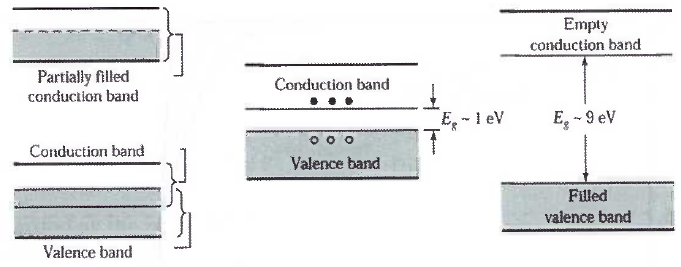
\includegraphics[width=1\textwidth]{ressources/bandgap.png}
  \caption{Schematische Darstellung des Bändermodells \cite{SZE}.}
  \label{bänder}
\end{figure}

Durch thermische Anregung von Elektronen im Valenzband ist es möglich, dass diese ins Leitungsband übergehen. Bei einem Isolator ist die Energiedifferenz der beiden Bänder ($E>\SI{4}{\electronvolt}$ \cite{SZE}) so groß, dass das Elektron trotz thermischer Anregung nicht in das Leitungsband übergehen kann. Im Gegensatz dazu ist die Energiedifferenz bei einem elektrischen Leiter so gering, dass Elektronen ohne externe Anregung in das Leitungsband angeregt werden können. Die Bandlücke eines Halbleiters liegt je nach Material und Dotierung im Bereich von $\SI{0,1}{\electronvolt}<E<\SI{4}{\electronvolt}$ \cite{SZE}. Somit wird ein kontrollierter Übergang, induziert durch eine externe Anregung, in dem Halbleiter ermöglicht.

 Des Weiteren werden Halbleiter in Element,-
Verbindungs,- und organische Halbleiter unterteilt. Innerhalb des Versuches wird
jedoch nur Silizium, also ein Elementhalbleiter, untersucht. Um die Leitfähigkeit
eines Halbleiters zu erhöhen können Fremdatome eingebracht werden, diesen Vorgang wird Dotierung genannt.


\subsection{p- und n- Halbleiter}
Der Elementhalbleiter Silizium gehört der vierten Hauptgruppe an und besitzt somit
vier Valenzelektronen. Zur Dotierung von Silizium eignen sich Atome mit drei oder
fünf Valenzelektronen. Dabei wird je nach Art der Dotierung zwischen
p-Typ (Dotierung mit Fremdatomen der dritten Hauptgruppe) und n-Typ (fünfte Hauptgruppe)
unterschieden.

Bei p-Typ Halbleitern wird ein Fremdatom der dritten Hauptgruppe eingefügt,
typische Dotierungsverhältnisse sind $10^{4-7}$ Si-Atome zu einem Fremdatom.
Durch die Dotierung fehlt ein Elektron in den kovalenten Bindungen, es entsteht ein
bewegliches Loch. Das Loch kann durch Elektroneneinfang wieder gefüllt werden,
deswegen werden solche Fremdatome auch als Akzeptoren bezeichnet.

Die n-Typ Halbleiter zeichnen sich durch eine Dotierung mit Elementen der
fünften Hauptgruppe aus. Bei einer solchen Dotierung entsteht ein Elektronenüberschuss
und pro dotiertes Fremdatom kommt es zu einem zusätzlichen Leitungselektron. Aufgrund
der Abgabe des Leitungselektron an das Gitter wird hier von einem Donator gesprochen.

\subsection{Der pn- Übergang}
An der Grenzfläche zwischen einem n- und einem p-dotierten Halbleiter bildet sich ein sogenannter pn-Übergang.
Der Überschuss an Elektronen aus dem n-dotierten Bereich und Überschuss der Löcher aus dem p-dotierten Bereich rekombinieren im Grenzbereich.
Zurück bleiben positiv bzw negativ ionisierte Atome, die durch ein sich aufbauendes elektrisches Feld, weitere Diffusion freie Ladungsträger unterbinden.
Dieser Bereich, in dem sich keine freien Ladungsträger mehr befinden, wird Depletionszone genannt. Ihre Dicke $d(U)$ hängt von der
dielektrischen Konstante des Halbleiters ab und kann mit
Hilfe der extern angelegten Spannung $U$ reguliert werden:
\begin{equation}
    \label{depl}
    d(U)=\sqrt{ \frac{ 2 \epsilon (U_D +U ) }{e N_\text{eff}}}.
\end{equation}
Des Weiteren hängt die Dicke von der Diffusionsspannung $U_D$ im dynamischen Gleichgewicht,
der Elementarladung $e$ und von der Anzahl der effektiven Ladungsträgerdichte ab. Die
effektive Ladungsträgerdichte ist ein Verhältnis der Dotierungskonzentrationen von
Donatoren $N_D$ und Akzeptoren $N_A$:
\begin{align}
	N_\text{eff}=\frac{N_D N_A}{N_D +N_A}\;.
\end{align}

Für exakte Messergebnisse im späteren Verlauf, ist es notwendig die Depletionszone zu maximieren. Eine weitere Ausdehnung dieser Zone, kann durch anlegen einer externen Spannung realisiert werden. Diese ist im Allgemeinen so groß $(U\gg U_\text{D})$, dass der Ausdruck \eqref{depl}
sich vereinfachen lässt zu:
\begin{equation}
    \label{dicke}
    d(U)=\sqrt{ \frac{ 2 \epsilon U }{e N_\text{eff}}}.
\end{equation}
Durch einsetzen der Spannung $U_\text{dep}$, lässt sie sich umformen zu
\begin{equation}
    U_\text{dep}=\frac{q}{2 \epsilon} N_\text{eff}D^2 \:.
\end{equation}
Liegt die externe Spannung im Bereich $ U\geq U_\text{dep}$ entspricht die dicker der Depletionszone der Sensordicke $D$ und wächst somit nicht weiter an.
Für Spannungen im Bereich $U<U_\text{dep}$ gilt die Näherung:

\begin{equation}
    \label{depsu}
d(U)=D\sqrt{\frac{U}{U_\text{dep}}}\:.
\end{equation}

Bei einer sogenannte IV-Kurve kann die Ausbildung der Depletionszone beobachtet werde. Hierbei wird der Leckstrom in Abhängigkeit der angelegten externen Spannnung gemessen. In Abbildung \ref{IVKurve} ist eine typische IV-Kurve dargestellt.

\begin{figure}[H]
  \centering
  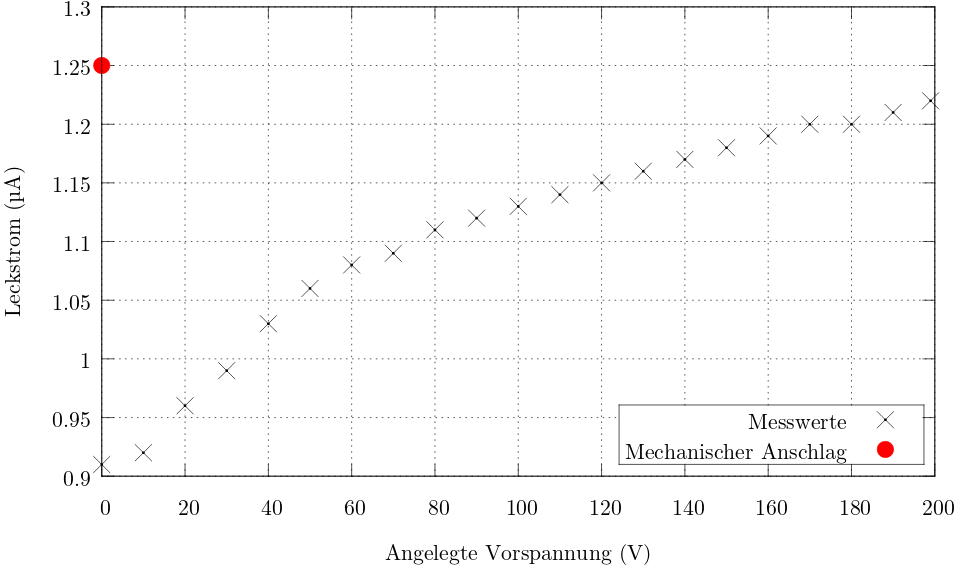
\includegraphics[width=0.7\textwidth]{ressources/IV.png}
  \caption{Typischer Verlauf einer IV-Kurve \cite{skript}.}
  \label{IVKurve}
\end{figure}

Bei zunächst kleinen Spannung steigt der Leckstrom, da sich die Depletionszone vergrößert und somit immer mehr Sensormaterial erschlossen wird. Nach dem erreichen der Depletionsspannung behält die Depletionszone eine konstante Größe, weshalb auch der Leckstrom nur noch leicht aufgrund thermische Fluktuation und der immer höheren angelegten Spannung steigt. Der Übergang zwischen den beiden Kurvenabschnitten stellt ein Maß für die Depletionsspannung dar. Genauere Messungen können mit der Aufnahme eine CV erfolgen.  

\subsection{Radioaktiver Zerfall}
Zerfällt ein instabiler Atomkern, entsteht $\alpha$-, $\beta$- oder $\gamma$-Strahlung, die ionisierend auf Materie wirkt. Die Zerfallsrate eines instabilen Materials, auch Quelle genannt, beschreibt mit der Einheit Bq $= [\frac{1}{s}]$ die Anzahl der Zerfälle pro Sekunde. Die aktuelle Aktivität der Quelle kann mit Hilfe der Aktivität $A_0$ zu einem bekannten Zeitpunkt und der Zerfallskonstante $\lambda$ wie folgt bestimmt werden:


\begin{equation}
    \label{lambda}
    A=A_0 e^{-\lambda t} \;.
\end{equation}

In diesem Versuch wurde eine $\ce{^{90}_{}Sr}$-Quelle verwendet. Diese ist ein reiner Gamma-Strahler, bei dem ein Neutron in ein Proton, ein Elektron und ein Antielektronneutrino zerfällt. Ein typisches Elektronenspektrum ist in Abbildung \ref{beta} dargestellt.

\begin{figure}[H]
  \centering
  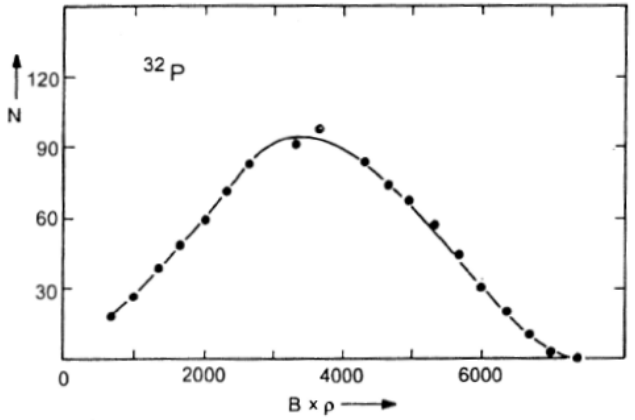
\includegraphics[width=0.7\textwidth]{ressources/beta.png}
  \caption{Typisches Elektronenspektrum einer $\beta$-Quelle \cite{skript}.}
  \label{beta}
\end{figure}

Das Strontium zerfällt zunächst in einem reinen $\beta$-Zerfall in Yttrium mit einer Halbwertszeit $\tau$ von etwa 29 Jahren. Yttrium zerfällt weiter mit einer Halbwertszeit $\tau$ von 2,5 Tagen in Zirkonium, wobei Zirkonium den stabilen Endzustand der Zerfallskette darstellt. Die Wechselwirkung der Elektronen mit der Materie im Detektor wird im folgenden Kapitel diskutiert.

\subsection{Wechselwirkung von Teilchen mit Materie}
In diesem Versuch werden zum einen ein Laser und zum anderen eine $\beta$-Quelle als Signalquelle zur Vermessung des Streifensensors verwendet. Somit werden in diesem Kapitel die Wechselwirkung von Photonen und Elektronen mit Materie genauer betrachtet.\\

Bis zu einer Energie von $E_\gamma \approx \SI{25}{\kilo\electronvolt}$ \cite{blub} eines Photons dominiert der Photoeffekt. Bei diesem überträgt ein einfallendes Photon seine komplette Energie auf ein Hüllenelektron der innersten Schalen. Ist die Energie des Photons größer als die Bindungsenergie des Elektrons, wird dieses ausgelöst. Die verbleibende Energie wird in Form von kinetischer Energie vom Elektron weggetragen. Infolge dessen nimmt ein Elektron aus einer höheren Schale des Platz des ausgelösten Elektrons ein, wobei, aufgrund der Energiedifferenz, ein Photon entsteht.\\

Ab einer Energie von $E_\gamma \approx \SI{25}{\kilo\electronvolt}$ \cite{blub} bis zu einer Energie von $E_\gamma \approx \SI{13}{\mega\electronvolt}$ \cite{blub} überwiegt der Comptoneffekt. Dieser beschreibt den elastischen Stoß eines einfallenden Photons mit einem Elektron. Diese Kollision verursacht einen Energieverlust des Elektrons, der von dem Elektron in Form von kinetischer Energie aufgenommen wird. Durch den Energieverlust entsteht eine Wellenlängenänderung bzw. Frequenzänderung des Photons.\\

Darüber hinaus, ab einer Energie von $E_\gamma \approx \SI{13}{\mega\electronvolt}$ \cite{blub} dominiert der Effekt der Paarbildung. Hierbei zerfällt ein Photon in Anwesenheit eines Stoßpartners, meist einem Atomkern, in ein Elektron und ein Positron. Für die Wechselwirkung mit einem Elektron benötigt das Photon die minimale Energie $E_{min}=4m_ec^2$ und bei der Wechselwirkung mit einem Kern eine Energie von $E_{min}=2m_ec^2$. Bei diesen Energien erhalten die entstandenen Teilchen jedoch keine kinetische Energie weshalb es zu einer Paarvernichtung kommt. \\

Bei der Wechselwirkung von geladenen Teilchen, hier Elektronen der $\beta$-Quelle mit Hüllenelektronen, entsteht Bremsstrahlung. Aufgrund des kleineren Energieübertrags entsteht im weiteren Verlauf ein kontinuierliches Spektrum. Mit der Bethe-Bloch-Formel  

\begin{equation}
    \label{Bloch}
    \left< -\frac{\text{d}E}{\text{d}x}\right>=Kz^2\frac{Z}{A}\cdot \frac{1}{\beta^2}\left(\frac{1}{2}\ln{\left(\frac{2m_ec^2\beta^2\gamma^2W_{max}}{I^2}\right)}-\beta^2-\frac{\delta(\beta\gamma)}{2}\right)
\end{equation}
wird der mittlere Verlust schwerer Teilchen durch Kollision pro Längeneinheit beschrieben, wobei diese nur im Bereich von $0,1 \leq \gamma\beta \leq 1000$ gilt. Für die Betrachtung von Elektronen müssen weitere Näherungen vorgenommen werden, siehe \cite{skript}. Mit den spezifischen Parametern des Aufbaus, ergibt sich eine mittlere Energiedeposition von \SI{3.88}{\mega\electronvolt\per\centi\meter}.

\subsection{Energieverteilung im Sensor}
Infolge des zentrales Grenzwertsatzes folgt der deponierten Energie von Elektronen im Silizium einer Gaußverteilung. Dabei wird davon ausgegangen, dass die Elektronen ihre komplette Energie im Sensor deponieren, welches nur durch eine hinreichende Sensordicke gewährleistet ist. Der in diesem Versuch verwendete Silizium-Streifen-Sensor misst eine Dicke von $\SI{300}{\micro\meter}$ und ist somit nicht ausreichend groß genug, damit eine vollständige Energiedeposition stattfinden kann. Durch diesen Umstand ist der zentrale Grenzwertsatz nicht mehr anwendbar. Durch den Umstand, dass auch die entstehenden Sekundärelektronen nicht komplett abgebremst werden können, entsteht eine asymmetrische Energieverteilung. Diese gleicht einer Landauverteilung. Zusätzlich ist zu beachten, dass die verwendete $\beta$-Quelle kein monoenergetisches Spektrum aufweißt, wodurch eine optimale Beschreibung der Energiedeposition im Silizium durch eine mit einer Gaußverteilung gefalteten Landauverteilung zustande kommt. Diese Verteilung ist für einen dünnen Sensor und typischer Elektronenenergie in Abbildung \ref{Verteilung} dargestellt.

\begin{figure}[H]
  \centering
  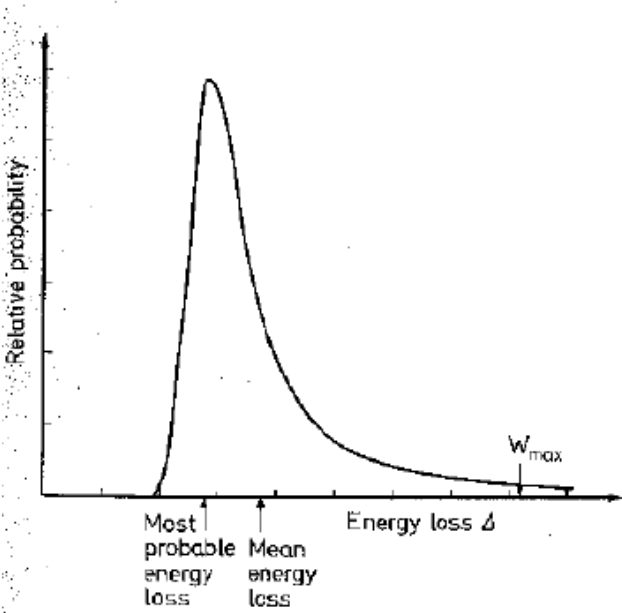
\includegraphics[width=0.7\textwidth]{ressources/Verteilung.png}
  \caption{Typische Energieverteilung in einem dünnen Sensor. \cite{skript}}
  \label{Verteilung}
\end{figure}


Da die Verteilung in ADC Counts angegeben wird, müssen diese zunächst in Energien der Einheit $eV$ umgerechnet werden. Diese erfolgt mit Kalibrationsmessung, bei der mit Hilfe eines Polynoms 4.Ordnung ein Zusammenhang zwischen ADC Counts und Pulsen bestimmt wird. Multipliziert mit der Energie zur Entstehung eines Elektron-Loch-Paars in Silizium, ergibt sich die Energie in der Einheit $eV$. 



\subsection{Noise}
\label{noise}
Bedingt durch die Ausleseelektronik des Sensors und durch den Sensor selbst entstehen sogenannte Störsignale. Diese verfälschen das benötigte Messsignal oder auch ADC($i$,$k$) Counts genannt. Dabei ist das Signal abhängig von dem betrachteten Streifen ($i$) und dem Eingangssignal ($k$). In Gleichung \ref{ADC} ist der Bezug zwischen dem ursprünglichen Signal und den ADC($i,k$) Counts beschrieben.

\begin{equation}
\label{ADC}
\text{ADC}(i,k)=P(i)+D(k)+\text{Signal}(i,k)\;.
\end{equation}

Pedestals $P(i)$ und der Common Mode Shift $D(k)$ sind dabei die angesprochenen Signalstörungen, die das Signal fälschlicherweise erhöhen. Pedestals beschreiben das Grundrauschen oder den Signaloffset eines Sensors in Abhängigkeit des Streifens. Dieses wird somit ohne externes Signal vermessen. Die Pedestals berechnen sich dann wie folgt:
\begin{equation}
    \label{peds}
    \text{P}(i)=\frac{1}{N}\sum_i^{N} \text{ADC}(i,k).
\end{equation}
Über die Summe alle Signale, die fälschlicherweise gemessen werden, wird summiert und anschließend der Mittelwert gebildet. Somit sind die Pedestals nur noch abhängig von dem betrachteten Streifen $i$. Der Common Mode Shift $D(k)$ bezeichnet eine Signalstörung bei der Verarbeitung eines Events, welches jeden Streifen betrifft. Berechnet wird diese wie folgt:
\begin{equation}
    \label{common}
    D(k)=\frac{1}{128}\sum_{i=1}^{128}(ADC(i,k)-P(i)).
\end{equation}
Aus den zuvor beschriebenen spezifisches Signalstörungen wird mit dem sogenannten Noise eine Größe zur allgemeinen und zusammenfassenden Beschreibung der Signalstörungen jedes Streifens berechnet. Dieses erfolgt mittels dem quadratischen Mittelwert der ADC Counts nach Abzug des Pedestals und des Common Mode Shifts.
\begin{equation}
    \label{noise}
    \text{Noise}=\sqrt{\frac{1}{N-1}\sum_{k=1}^{N}( \text{ADC}(i,k)-\text{P}(i)-\text{D}(k))^2. }
\end{equation}

Mit der berechneten Noise des Sensors wird ein Signal-to-Noise-Cut durchgeführt werden. Hierfür wird das Verhältnis zwischen dem Signal und dem entstandene Noise gebildet. Überwiegt dabei das Signal das Rauschen um das fünffache, wird das Signal weiter analysiert. 

% 2x2 Plot
% \begin{figure*}
%     \centering
%     \begin{subfigure}[b]{0.475\textwidth}
%         \centering
%         \includegraphics[width=\textwidth]{Abbildungen/Schaltung1.pdf}
%         \caption[]%
%         {{\small Schaltung 1.}}
%         \label{fig:Schaltung1}
%     \end{subfigure}
%     \hfill
%     \begin{subfigure}[b]{0.475\textwidth}
%         \centering
%         \includegraphics[width=\textwidth]{Abbildungen/Schaltung2.pdf}
%         \caption[]%
%         {{\small Schaltung 2.}}
%         \label{fig:Schaltung2}
%     \end{subfigure}
%     \vskip\baselineskip
%     \begin{subfigure}[b]{0.475\textwidth}
%         \centering
%         \includegraphics[width=\textwidth]{Abbildungen/Schaltung4.pdf}    % Zahlen vertauscht ... -.-
%         \caption[]%
%         {{\small Schaltung 3.}}
%         \label{fig:Schaltung3}
%     \end{subfigure}
%     \quad
%     \begin{subfigure}[b]{0.475\textwidth}
%         \centering
%         \includegraphics[width=\textwidth]{Abbildungen/Schaltung3.pdf}
%         \caption[]%
%         {{\small Schaltung 4.}}
%         \label{fig:Schaltung4}
%     \end{subfigure}
%     \caption[]
%     {Ersatzschaltbilder der verschiedenen Teilaufgaben.}
%     \label{fig:Schaltungen}
% \end{figure*}
